\documentclass[10pt,twocolumn]{article}

% Packages
\usepackage{graphicx} % For figures
\usepackage{amsmath, amssymb} % Math symbols
\usepackage{booktabs} % Tables
\usepackage{hyperref} % Hyperlinks
\usepackage{caption} % Better captions
\usepackage{geometry} % Page layout
\geometry{a4paper, margin=1in}

\usepackage{mathtools}
\usepackage{amsthm}
\usepackage{enumerate}
\usepackage{fontawesome}
\usepackage{multirow}
\usepackage[many]{tcolorbox}
\usepackage{mdframed}
\usepackage{hyperref}
\usepackage[textsize=tiny]{todonotes}
\usepackage{tikz}
\usetikzlibrary{shapes.geometric, arrows}
\tikzstyle{startstop} = [rectangle, rounded corners, minimum width=3cm, minimum height=1cm,text centered, draw=black, fill=red!30]
\tikzstyle{process} = [rectangle, minimum width=3cm, minimum height=1cm, text centered, draw=black, fill=orange!30]
\tikzstyle{arrow} = [thick,->,>=stealth]
\usepackage{enumitem}   

% Title Information
\title{Case for a unified surrogate modelling framework in the age of AI}
\author{Elizaveta Semenova \\ Imperial College London \\ \texttt{e.semenova@imperial.ac.uk}}
\date{}

\begin{document}

\maketitle

\begin{abstract}
Surrogate models are widely used in natural sciences, engineering, and machine learning to approximate complex systems and reduce computational costs. However, the current landscape lacks standardisation across key stages of the pipeline, including data collection, sampling design, model class selection,  evaluation metrics, and downstream task performance analysis. This fragmentation limits reproducibility, reliability, and cross-domain applicability. The issue has only been exacerbated by the AI revolution and a new suite of surrogate model classes that it offers. In this position paper, we argue for the urgent need for a unified framework to guide the development and evaluation of surrogate models. We outline essential steps for constructing a comprehensive pipeline and discuss alternative perspectives, such as the benefits of domain-specific frameworks. By advocating for a standardised approach, this paper seeks to improve the reliability of surrogate modelling, foster cross-disciplinary knowledge transfer, and, as a result, accelerate scientific progress.
\end{abstract}

%%%%%%%%%%%%%%%%%%%%%%%%%%%%%%%%%%%%%%%%%%%%%%%%%%
%%%%%%%%%%%%%%%%%%%%%%%%%%%%%%%%%%%%%%%%%%%%%%%%%%
% Intro
%%%%%%%%%%%%%%%%%%%%%%%%%%%%%%%%%%%%%%%%%%%%%%%%%%
%%%%%%%%%%%%%%%%%%%%%%%%%%%%%%%%%%%%%%%%%%%%%%%%%%
\section{Introduction}
Surrogate modelling has become an indispensable tool for approximating complex computational systems across diverse fields, including engineering, natural sciences, machine learning, and artificial intelligence. By serving as cost-effective substitutes for expensive simulations or experiments, surrogate models (SMs) enable researchers to explore design spaces, optimise processes, and make predictions with significantly reduced computational overhead \cite{forrester2008}.

The landscape of surrogate modelling has evolved dramatically in recent years, driven in large part by advances in artificial intelligence. Traditional methodologies, such as nonparametric statistical methods, \textit{e.g.}, Gaussian processes \cite{rasmussen2006, gramacy2020surrogates, marrel2024probabilistic}, splines \cite{audoux2018surrogate}, hierarchical or mixed-variable models \cite{saves2024smt}), and polynomial chaos expansion \cite{novak2018polynomial}, have been complemented—and in some cases, outpaced by modern AI-driven approaches. These include neural network-based surrogates \cite{hua2024learning}, physics-informed neural networks \cite{raissi2019}, Bayesian neural networks \cite{li2023study}, and conditional deep generative models \cite{silionis2023conditional}. Emerging paradigms such as world models \cite{ha2018world} and digital twins \cite{sharma2022digital} are further reshaping the field, pushing the boundaries of what surrogate models can achieve.

However, this rapid proliferation of AI-driven methods has led to a fragmented landscape. Application domains often rely on bespoke approaches, complicating performance evaluation and making it challenging to establish best practices. Key decisions—such as whether a model should be deterministic or stochastic, whether it should incorporate domain knowledge, and how its quality should be assessed—are frequently handled inconsistently or overlooked entirely. These inconsistencies hinder reproducibility and hinder cross-disciplinary knowledge transfer, limiting the broader impact of surrogate modelling advancements.

\begin{tcolorbox}[
colback=blue!5!white, % Use custom teal color
colframe=blue!75!black, % Use custom teal color for frame
boxrule=0.5mm, % Thickness of the frame
arc=3mm, % Corner rounding
left=2mm, % Left padding
right=2mm, % Right padding
top=2mm, % Top padding
bottom=2mm % Bottom padding
]
{\fontsize{10}{20}\selectfont \faLightbulbO
}\hspace{2mm}~%
\textbf{Position statement:} In the age of AI, the field of surrogate modelling urgently needs a unified framework for training and evaluation to address current inconsistencies, foster reproducibility, and spur cross-disciplinary translation.
\end{tcolorbox}

The primary objective of this paper is to make a case for such a \textbf{unified framework}, particularly in light of the transformative impact of AI on surrogate modelling. A unified framework would standardise critical steps in the pipeline, including input data formats, sampling design for data collection, model selection, training loss functions, evaluation metrics, uncertainty quantification, and performance on downstream tasks. By doing so, it would enhance the reliability of surrogate models and facilitate cross-domain collaborations, ensuring that advancements in one field can be effectively translated to others \cite{willard2020}.

The need for standardisation is particularly pressing given the expanding use of SMs in critical applications such as climate modelling \cite{camps-valls2019, borisova2023surrogate, durand2024data, aretz2024multifidelity}, electric motor engineering \cite{cheng2024review}, reservoir development \cite{zhao2024review}, epidemiology \cite{pereira2021deep, abbottevaluating, schmidt2024towards, angione2022using}, drug development, protein design \cite{gruver2021effective}, physical sciences \cite{wu2025developing}, groundwater modelling \cite{asher2015review, razavi2012}, wildfire nowcasting \cite{cheng2023generative}, and sea-ice modelling \cite{finn2024generative}. Without a common framework, it is difficult to ensure that SMs are both robust and interpretable, particularly as their use expands to high-stakes domains.

By proposing a structured and comprehensive framework, this paper seeks to catalyse a shift toward more consistent and transparent practices in surrogate modelling. 

The remainder of the paper is organised as follows: Section~\ref{sec:proposed} introduces the proposed unified framework and its key components (with a link to an appendix evaluating 20 publications against the framework); Section~\ref{sec:alternative-views} presents alternative perspectives and addresses concerns about standardisation; and Section~\ref{sec:discussion} summarises the contributions and offers a call to action for the community.

%%%%%%%%%%%%%%%%%%%%%%%%%%%%%%%%%%%%%%%%%%%%%%%%%%
%%%%%%%%%%%%%%%%%%%%%%%%%%%%%%%%%%%%%%%%%%%%%%%%%%
% Proposed framework
%%%%%%%%%%%%%%%%%%%%%%%%%%%%%%%%%%%%%%%%%%%%%%%%%%
%%%%%%%%%%%%%%%%%%%%%%%%%%%%%%%%%%%%%%%%%%%%%%%%%%
\section{Proposed unified framework}
\label{sec:proposed}

\begin{figure*}[ht]
\centering
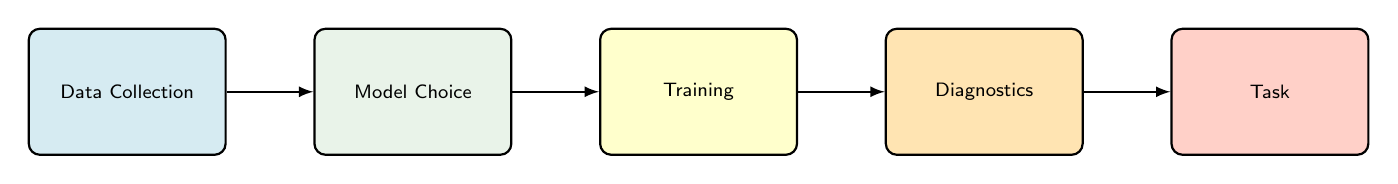
\begin{tikzpicture}[
    font=\sffamily\scriptsize,
    node distance=1.1cm,
    >=latex, % Use default latex arrow tip
    line/.style={draw, -latex, thick},
    block/.style={
        rectangle,
        rounded corners,
        draw=black,
        thick,
        minimum width=2.5cm,
        minimum height=1.6cm,
        align=center
    }
]

% Define Colors
\definecolor{datacolor}{RGB}{70,130,180}    % Steel Blue
\definecolor{modelcolor}{RGB}{34,139,34}    % Forest Green
\definecolor{traincolor}{RGB}{255,215,0}    % Gold
\definecolor{evalcolor}{RGB}{255,140,0}     % Dark Orange
\definecolor{taskcolor}{RGB}{178,34,34}     % Firebrick

\definecolor{datacolor}{RGB}{173,216,230} % Light blue
%\definecolor{modelcolor}{RGB}{144,238,144} % Light green
\definecolor{traincolor}{RGB}{255,255,153} % Light yellow
\definecolor{evalcolor}{RGB}{255,165,0}   % Orange
\definecolor{taskcolor}{RGB}{255,99,71}   % Tomato red

% Main Nodes
\node[block, fill=datacolor!50] (data) {Data Collection};
\node[block, fill=modelcolor!10, right=of data] (model) {Model Choice};
\node[block, fill=traincolor!50, right=of model] (training) {Training};
\node[block, fill=evalcolor!30, right=of training] (evaluation) {Diagnostics};
\node[block, fill=taskcolor!30, right=of evaluation] (tasks) {Task};

% Connections Between Main Nodes
\draw[line] (data.east) -- (model.west);
\draw[line] (model.east) -- (training.west);
\draw[line] (training.east) -- (evaluation.west);
\draw[line] (evaluation.east) -- (tasks.west);

\end{tikzpicture}
\caption{Overview of the proposed unified surrogate modelling pipeline}
\label{fig:unified_pipeline}
\end{figure*}



In this section, we propose a unified framework for surrogate modelling that articulates standardised practices for data collection, model selection, training, evaluation, and uncertainty quantification. Increasingly, \textbf{AI-driven} or \textbf{machine learning} approaches—such as large-scale deep neural architectures or generative models—are crucial to pushing the frontiers of surrogate modelling across disciplines. At its core, the framework emphasises modularity so that specific stages may be tailored to domain requirements while preserving the consistency needed for reproducibility, rigorous evaluation, and cross-disciplinary transfer. Figure \ref{fig:unified_pipeline} presents the overview of the pipeline, and in subsequent sections we detail its components.

\subsection{Data collection and generation}
The quality and representativeness of training data are critical to the success of SMs. Poorly collected or non-representative data can lead to biased models, inaccurate
predictions, and ultimately, flawed decision-making \cite{bradley2021unrepresentative}. We suggest two considerations within the data collection routine: input data mode and sampling design. We also emphasise the need for standardised input formats.

\subsubsection{Two modes of input data}
\label{sec:data-modes}
 We consider two main modes of data: (i) collected from real-life systems and (ii) generated by computational systems, including both offline (“pre-generated”) and online (“on-the-fly”) simulations. 
 
 \textbf{(i) Real-life data.} These arise from physical experiments or observational campaigns (\textit{e.g.}, sensor readings for climate studies, lab measurements in drug discovery, clinical trails data). They are typically stored for later use, posing challenges in quality control, bias detection, and ensuring metadata completeness. 
 
 \textbf{(ii) Computational data.} These come from simulators or numerical models. One can adopt an offline route, where simulations are run in batches and stored, or an online route, where new samples are generated adaptively, guided by error metrics or active learning strategies. Emerging \textbf{AI-based simulators}, such as large neural PDE solvers or physics-informed neural networks (PINNs), can further serve as cost-effective data generators to pre-train surrogates at scale.

\subsubsection{Standardised data formats}
\label{sec:data-formats}
To enhance interoperability, the framework advocates adopting domain-specific and general-purpose data standards. Examples include NetCDF for climate science \cite{rew1990netcdf}, SMILES in drug discovery \cite{weininger1988smiles}, HDF5 for engineering \cite{folk1999hdf}, Parquet for large tabular data \cite{weber2022parquet}, or GeoTiff \cite{ritter1997geotiff} for raster geographic images. Embedding thorough metadata (\textit{e.g.}, CF Conventions \cite{eaton2003netcdf} or Dublin Core \cite{weibel1997dublin}) ensures transparency in data sources and fosters reproducibility. Such standardisation also paves the way for \textbf{foundation-model-based} data preprocessing or data augmentation approaches, which require consistent formatting across diverse sources.

\subsubsection{Sampling design}
\label{sec:sampling}
Sampling choices directly impact data representativeness, computational costs, and the generalisability of the resulting surrogate model \cite{kamath2022intelligent}. Two straightforward strategies are \textbf{random sampling}, which draws points uniformly at random from the input domain, and \textbf{grid sampling}, which places points on a fixed mesh to ensure uniform coverage in low-dimensional spaces. While these basic approaches can be easy to implement or interpret, they are often suboptimal in higher dimensions: random sampling may leave significant gaps or clusters, and grid sampling rapidly becomes infeasible as dimensionality grows. 

A variation of random sampling involves drawing points from a \textbf{non-uniform prior distribution}, which can be particularly useful when prior knowledge about the input domain is available. For instance, if certain regions of the input space are known to be more influential or relevant, sampling can be biased towards these areas. However, the notion of `uniformity' becomes complex in nonlinear systems, where the relationship between inputs and outputs may distort the perceived uniformity of the sampling. In such cases, uniformity in the input space does not necessarily translate to uniformity in the output space, making it challenging to ensure representative sampling without careful consideration of the system's nonlinear dynamics.

Consequently, more sophisticated \emph{space-filling} approaches are commonly used, including \textbf{Latin hypercube sampling (LHS)}, \textbf{Sobol} or \textbf{Halton sequences}, and \textbf{orthogonal array}-based designs. For many problems, \textbf{adaptive sampling} is especially powerful: once an initial batch is collected (\textit{e.g.,} via LHS), the model directs further sampling to regions of high uncertainty or high importance, effectively balancing exploration and exploitation in the sampling process.


\textbf{AI-driven sampling.} An emerging trend is to leverage AI and especially \textbf{reinforcement learning (RL)} to adaptively choose sample locations that maximise information gain. In RL-based approaches, an agent (\textit{e.g.}, a policy network) learns to sequentially propose inputs that reduce SM uncertainty or improve downstream objectives \cite{cestero2024building}. Ulike traditional methods with fixed heuristics, RL agents dynamically adapt the surrogate model's evolving behaviour \cite{arulkumaran2017deep}. This builds on foundational concepts in \textbf{active learning (AL)}, where iterative sampling targets regions of high model uncertainty (e.g., query-by-committee or entropy-based methods)~\cite{settles2009active}, and \textbf{Bayesian optimization (BO)}, which uses acquisition functions (\textit{e.g.}, expected improvement, upper confidence bound) to balance exploration and exploitation~\cite{shahriari2015taking}. However, RL generalises these ideas by learning the sampling strategy itself. While RL-based methods excel in adaptability, they require careful reward function design and significant upfront training data. In contrast, BO remains more sample-efficient for low-dimensional problems~\cite{garnett2023bayesian}. Emerging solutions include meta-learning for fast adaptation across tasks~\cite{volpp2019meta}. Such approaches as BO, AL and RL mitigate the ``curse of dimensionality'' by focusing computational resources on sparse, high-impact regions.


\begin{tcolorbox}[
    colback=green!5!white,
    colframe=green!75!black,
    boxrule=0.5mm,
    arc=3mm,
    left=2mm,
    right=2mm,
    top=2mm,
    bottom=2mm
]
    {\fontsize{10}{20}\selectfont \faCog}\hspace{2mm}~%
    \textbf{Data collection guideline}
    \begin{itemize}[label=\faCheck, labelsep=0.5em]
        \vspace{-0.2cm}
        \item Use standardised file formats.
        \vspace{-0.2cm}
        \item Select sampling strategy.
        \vspace{-0.2cm}
    \item Collect ``offline" or ``on-the-fly" data.
\end{itemize}
\end{tcolorbox}


\subsection{Model class selection}
\label{sec:model-class-selection}

Selecting an appropriate model class profoundly impacts predictive performance, interpretability, and computational feasibility. This framework distinguishes models by their \textbf{fidelity} level, \textbf{deterministic vs.\ stochastic} nature, \textbf{parametric vs.\ nonparametric} assumptions, and whether they can \textbf{condition} on auxiliary variables.

\subsubsection{Fidelity level}
Multi-fidelity modelling leverages a hierarchy of simulation or measurement fidelities. Low-fidelity approximations (cheaper but coarser) guide the model to promising regions; high-fidelity counterparts refine solutions. This approach can reduce the number of expensive high-fidelity runs by intelligently allocating computational resources \cite{ conti2024multi}.

\subsubsection{Deterministic vs.\ stochastic SMs}
\label{sec:det-vs-stoch}
\textbf{Deterministic surrogates} (\textit{e.g.}, splines \cite{audoux2018surrogate}, feed-forward neural networks) produce single-valued outputs. They suit deterministic phenomena and can be sufficiently quickly optimised. \textbf{Stochastic surrogates} output probability distributions, valuable for \emph{stochastic simulators} (\textit{e.g.}, epidemiological agent-based models \cite{pereira2021deep}) or if uncertainty quantification is paramount. \textbf{Probabilistic neural networks}, Gaussian processes, or modern \textbf{deep generative models} like diffusion models \cite{finn2024generative} capture and propagate uncertainty from both data and model structure. When calibrating to real-world data, these surrogates provide a more complete picture of possible outcomes.

\subsubsection{Uncertainty quantification}
\label{sec:UQ}
Regardless of determinism vs.\ stochasticity, systematic \textbf{uncertainty quantification (UQ)} is vital. Ensemble methods (\textit{e.g.}, random forests), variational inference, and Bayesian techniques all provide uncertainty estimates around predictions. Advances in \textbf{deep ensembles} or \textbf{stochastic variational inference} enable tractable UQ even for large neural surrogates. UQ reveals where data are sparse, guiding adaptive sampling or trust regions for downstream tasks like optimisation.

\subsubsection{Parametric vs.\ nonparametric SMs}
\label{sec:parametric-vs-nonparametric}
\textbf{Parametric} surrogates (\textit{e.g.}\ polynomials, classical neural networks) assume a fixed functional form and tune a finite set of parameters, often excelling in high-dimensional or large-data scenarios. Recent parametric approaches include large-scale \textbf{transformer-based} surrogates that handle complex spatiotemporal data by learning global attention patterns \cite{li2024scalable}, including graph transformers \cite{feng2024novel}. Neural network architecture search is a significant step under the model selection umbrella.

By contrast, \textbf{nonparametric} models (\textit{e.g.}\ Gaussian processes) flexibly adapt to data without assuming a rigid functional family. They often outperform parametric methods in low-data regimes or when the underlying function class is unknown. However, they can be computationally expensive, especially as dataset sizes grow. Techniques such as sparse GPs and kernel approximations can mitigate these costs.

\subsubsection{Conditionality}
Many applications require \textbf{conditional} surrogates, which produce outputs conditioned on auxiliary inputs (\textit{e.g.}\ boundary conditions, environment states). Conditional deep generative models \cite{silionis2023conditional}, for instance, learn distributions $p(\mathbf{x} \mid \mathbf{c})$, enabling scenario-specific predictions and parameter inference.

\subsubsection{Additional Constraints}
\label{sec:additional-constraints}
Domain-specific constraints—physical, geometric, or monotonicity requirements—must be integrated to ensure realistic outputs. \textbf{Physics-informed neural networks (PINNs)} \cite{raissi2019} embed governing equations into the loss function, guaranteeing physically plausible predictions even with limited data. \textbf{Geometry-aware} surrogates \cite{oldenburg2022geometry} preserve topological properties, and \textbf{monotonic} surrogates \cite{sill1997monotonic} enforce known increasing/decreasing relationships.


\begin{tcolorbox}[
    colback=green!5!white,
    colframe=green!75!black,
    boxrule=0.5mm,
    arc=3mm,
    left=2mm,
    right=2mm,
    top=2mm,
    bottom=2mm
]
    {\fontsize{10}{20}\selectfont \faCog}\hspace{2mm}~%
    \textbf{Model class selection guideline}
    \begin{itemize}[label=\faCheck, labelsep=0.5em]
        \vspace{-0.2cm}
        \item Select fidelity level.
        \vspace{-0.2cm}
        \item Choose stochastic vs deterministic.
        \vspace{-0.2cm}
        \item Choose parametric vs nonparametric.
        \vspace{-0.2cm}
        \item Conditional or not.
        \vspace{-0.2cm}
        \item Incorporate domain-specific constraints.
\end{itemize}
\end{tcolorbox}


\subsection{Learning methods and loss functions}
\label{sec:loss-functions }

Training a surrogate model typically involves minimising a loss function to align its predictions with reference data while respecting any embedded domain constraints. However, \textbf{optimisation} is not the only paradigm; alternative approaches such as Bayesian inference, generalised Bayesian inference, reinforcement learning, and simulation-based methods can also be used, depending on the problem context and the nature of the surrogate.


\subsubsection{Loss functions for deterministic SMs}
For \textbf{deterministic} surrogates, common loss functions include negative log-likelihoods, corresponding to the modelled data type. This would be cross-entropy for classification, or, the mean squared error for regression in its simplest form; also mean absolute error, and Huber loss. 
% In scenarios where the model's performance varies significantly across the input space, \textbf{adaptive} losses can dynamically weight errors, emphasising regions where the model is uncertain or performs poorly. This is well suited in active learning loops, where the surrogate is iteratively refined based on its own predictions.

\subsubsection{Bayesian inference}
When uncertainty quantification is key, and/or prior knowledge is available, \textbf{Bayesian inference} is an indispensable tool, applicable to both deterministic and stochastic models. In this case, optimisation task is replaced with integration, and intricate sampling algorithms, such as Markov Chain Monte Carlo (MCMC) can be used.

\textbf{Generalised Bayesian inference} extends the Bayesian inference framework by relaxing the need for strict probabilistic interpretations of the loss function. Instead of relying solely on likelihood-based objectives, generalised Bayesian methods use task-specific loss functions, such as robust regression or classification losses, while maintaining a probabilistic interpretation of uncertainty. This flexibility makes generalised Bayesian inference useful in settings where traditional likelihood-based approaches are impractical or overly restrictive.

\subsubsection{Learning stochastic surrogates with generative AI}
For \textbf{stochastic} surrogates, Bayesian inference provides a principled framework for uncertainty quantification and model training. However, it might be computationally infeasible. Modern \textbf{deep generative (generative AI)} surrogates are often used in this case; they leverage objectives like the Evidence Lower Bound (ELBO) to learn latent representations of the data, enabling the model to capture complex, high-dimensional distributions. These methods combine the strengths of Bayesian inference with the expressive power of deep neural networks, making them well-suited for tasks such as generative modelling and uncertainty-aware prediction.

% Traditional Bayesian methods optimise objectives such as the negative log-likelihood (NLL) or Kullback-Leibler (KL) divergence to infer posterior distributions over model parameters. These methods are particularly effective when prior knowledge about the system is available and can be encoded into the model.



\subsubsection{Simulation-based inference}
In cases where explicit likelihoods are unavailable or intractable, \textbf{simulation-based inference} (SBI) frameworks provide a powerful alternative. SBI methods train surrogates by comparing synthetic data generated from simulations with real observations, bypassing the need for explicit likelihood evaluations. This approach is particularly useful in scientific domains where simulations are computationally expensive but provide a reliable source of data \cite{cranmer2020frontier}.

\subsubsection{Regularization and constrained optimisation}
To improve generalization and enforce domain-specific constraints, regularization techniques such as L1/L2 regularization or physics-informed penalty terms are often integrated into the loss function. Constrained optimisation methods can also be used to ensure that the surrogate respects physical laws or other domain-specific rules. For example, PINNs incorporate governing equations directly into the training process, enabling the surrogate to learn solutions that are consistent with known physical principles.

\subsubsection{Automated surrogate selection}
The process of selecting and tuning a surrogate model can be automated using AI-driven AutoML tools. These tools systematically explore hyperparameters, architectures, and model classes—such as neural networks, Gaussian processes, or ensemble methods—to identify configurations that balance accuracy, computational cost, and generalizability. By automating this search, AutoML pipelines reduce the need for manual trial-and-error, enabling researchers to focus on higher-level design and interpretation \cite{feurer2019hyperparameter}.


\begin{tcolorbox}[
    colback=green!5!white,
    colframe=green!75!black,
    boxrule=0.5mm,
    arc=3mm,
    left=2mm,
    right=2mm,
    top=2mm,
    bottom=2mm
]
    {\fontsize{10}{20}\selectfont \faCog}\hspace{2mm}~%
    \textbf{Learning methods guideline}: Select one of
    \begin{itemize}[label=\faCheck, labelsep=0.5em]
        \vspace{-0.2cm}
        \item Optimisation.
        \vspace{-0.2cm}
        \item Bayesian inference.
        \vspace{-0.2cm}
        \item Generalised Bayesian inference.
        \vspace{-0.2cm}
        \item Simulation-based inference.
\end{itemize}
\end{tcolorbox}


\subsection{Evaluation  metrics}
\label{sec:evaluation-metrics}
The framework distinguishes \emph{diagnostic} from \emph{task-based} evaluation. While evaluation metrics often mirror the training loss, they can diverge to evaluate broader aspects such as uncertainty quantification, robustness, and alignment with domain-specific goals. For instance, a likelihood-trained model may be evaluated using calibration metrics.

\subsubsection{Diagnostic evaluation - distributional similarity metrics}
When evaluating stochastic surrogate models, it is often necessary to compare the distribution of model outputs to the true data distribution. The \textbf{maximum mean discrepancy (MMD)} \cite{gretton2012kernel} is a kernel-based metric that quantifies the difference between two probability distributions. MMD is particularly useful for high-dimensional data and can detect subtle differences in distributions. Another powerful metric for comparing distributions is the Fréchet distance. In the context of generative models, it is often referred to as the \textbf{Fréchet Inception Distance (FID)} \cite{heusel2017gans} when applied to image data. Lower FD values indicate greater similarity between distributions. Another options is \textbf{sliced-Wasserstein (SW)}.

A comprehensive review of metrics applicable specifically to generative models is available in \cite{bischoff2024practical}.

\subsubsection{Diagnostic evaluation – simulation-based calibration}
\textbf{Simulation-based calibration (SBC)} \cite{talts2018validating} is a robust method for evaluating the calibration of Bayesian models, including stochastic surrogates. SBC involves generating synthetic datasets from the model’s prior predictive distribution, fitting the model to each dataset, and comparing the posterior distributions to the true parameters. A well-calibrated model should produce posterior distributions that are statistically consistent with the true parameters.

% \subsubsection{Diagnostic evaluation: distributional similarity \& calibration}
% \label{sec:diagnostic-eval}
% For \textbf{stochastic} surrogates, comparing generated vs.\ true data distributions is key. \textbf{Maximum mean discrepancy (MMD)} \cite{gretton2012kernel} or \textbf{Fréchet Inception Distance (FID)} \cite{heusel2017gans} are popular in high-dimensional settings (e.g.\ images). Simulation-based calibration (SBC) \cite{talts2018validating} tests the consistency of posterior samples with “true” parameters, ensuring well-calibrated models.

\subsubsection{Task-based evaluation}
Surrogate models often serve downstream tasks such as \textbf{Bayesian optimisation} \cite{shahriari2015taking} or \textbf{active learning} \cite{settles2009active}. Evaluating how well a surrogate drives these tasks is often more meaningful than raw predictive error alone. For instance, in Bayesian optimisation, metrics like \emph{regret}  measure how quickly the pipeline converges to an optimum. In uncertainty propagation or reliability analysis, \emph{coverage probability} may be more critical than MSE.

\begin{tcolorbox}[
    colback=green!5!white,
    colframe=green!75!black,
    boxrule=0.5mm,
    arc=3mm,
    left=2mm,
    right=2mm,
    top=2mm,
    bottom=2mm
]
    {\fontsize{10}{20}\selectfont \faCog}\hspace{2mm}~%
    \textbf{Diagnostics and evaluation guideline.}
    \begin{itemize}[label=\faCheck, labelsep=0.5em]
        \vspace{-0.2cm}
        \item Predictive performance.
        \vspace{-0.2cm}
        \item Distributional similarity.
        \vspace{-0.2cm}
        %\item Simulation-based calibration
        %\vspace{-0.2cm}
        \item Downstream task performance.
\end{itemize}
\end{tcolorbox}

\subsection{Benchmarks}
To foster reproducibility and fair model comparisons in surrogate modelling, especially in the age of AI, the community requires \emph{widely accepted} and \emph{systematically curated} benchmarks. Such resources should span different data types and application contexts---for instance, PDE solvers, fluid dynamics, epidemiological and climate datasets---and include standardised protocols, and comprehensive metadata. Structured and versioned benchmark suites (with explicit documentation of data origins and domain assumptions) would enable researchers to evaluate SMs under consistent conditions while tracing improvements over time. 

Publicly available challenge platforms, such as \textsc{OpenML} or Kaggle, could further promote best practices and highlight performance trade-offs across model families, aiding both newcomers and experts in benchmarking new innovations. Additionally, \emph{AI-driven benchmarking} strategies, where adaptive test sets or generative models dynamically challenge surrogates in previously unseen domains, may help reveal generalisation limits. By centralising these efforts within a unified framework, we can advance more reliable, transparent, and cross-domain-compatible surrogate modelling practices.


\subsection{Case studies}
To illustrate how existing research aligns with or diverges from our unified surrogate modelling framework, Appendix~\ref{appendix:case-studies} reviews 20 recent studies using SMs. Each study is mapped onto the key components of our pipeline. Overall, these case studies reveal both the versatility of surrogate modelling, evidenced by its diverse applications, and the fragmentation that occurs in practice. In particular, most works employ domain-specific data formats with minimal standardisation or metadata, and they show significant variation in sampling designs, often defaulting to basic or \textit{ad hoc} methods rather than adaptive approaches. Despite the widespread use of deterministic neural networks, models such as Gaussian processes and latent variable neural processes are less frequently adopted, and discussions of domain-specific constraints tend to be brief. Training typically relies on classical minimisation of MSE or RMSE, while Bayesian or simulation-based inference methods receive relatively little attention. Uncertainty quantification is similarly underutilised, despite the inherent complexity of applications like climate or agent-based modelling. Evaluation procedures tend to focus on pointwise error metrics, with only a few studies addressing distributional alignment or task-specific metrics. 

%%%%%%%%%%%%%%%%%%%%%%%%%%%%%%%%%%%%%%%%%%%%%%%%%%
%%%%%%%%%%%%%%%%%%%%%%%%%%%%%%%%%%%%%%%%%%%%%%%%%%
% Alternative views
%%%%%%%%%%%%%%%%%%%%%%%%%%%%%%%%%%%%%%%%%%%%%%%%%%
%%%%%%%%%%%%%%%%%%%%%%%%%%%%%%%%%%%%%%%%%%%%%%%%%%


\section{Alternative Views}
\label{sec:alternative-views}

While the proposed unified framework for surrogate modelling offers significant benefits, several alternative perspectives challenge its feasibility and desirability. Below, we address three key critiques, supported by real-world examples and literature, and provide counterarguments grounded in the framework’s design principles.

\subsection{Domain-specific needs outweigh cross-disciplinary benefits}  
The first possible critique point is that the surrogate modelling pipelines must remain domain-specific to accommodate unique requirements. For instance, in climate science \cite{watson2022climatebench}, uncertainty quantification must be prioritised. Similarly, in aerospace engineering, real-time performance and high-fidelity predictions are critical for design optimisation, as seen in the use of Gaussian processes for aerodynamic modelling \cite{forrester2008}. Domain-specific tools like the Surrogate Modelling Toolbox (SMT) \cite{saves2024smt} and physics-informed neural networks (PINNs) \cite{raissi2019} have demonstrated success by tailoring methods to narrow use cases.

This perspective holds that standardisation risks oversimplification, forcing researchers to adopt ill-fitting practices. For instance, in drug discovery, SMs must handle molecular representations like SMILES strings \cite{weininger1988smiles}, which are not easily transferable to other domains. Similarly, in epidemiology, agent-based models (ABMs) require stochastic surrogates to capture complex social dynamics \cite{angione2022using}, unlike deterministic physical systems governed by ordinary differential equations.

However, the proposed framework explicitly advocates for modularity, allowing domains to retain specialised components (\textit{e.g.}, climate-specific metadata standards) while harmonising core elements like evaluation metrics and uncertainty reporting. Cross-pollination between fields—such as adapting adaptive sampling from aerospace engineering \cite{raul2021surrogate} to wildfire modelling \cite{cheng2023generative}—demonstrates the untapped potential of shared methodologies. By providing a flexible yet consistent structure, the framework enables domain-specific adaptations without sacrificing interoperability.

\subsection{Technical and institutional barriers to adoption}
A second critique highlights practical challenges in retrofitting legacy systems. Many scientific communities rely on proprietary or highly specialised software. For example, groundwater modelling often uses finite difference approximation such as implemented in MODFLOW \cite{harbaugh2005modflow} or a finite element method, as used for example by FEFLOW \cite{diersch2013feflow, asher2015review}, i.e. legacy systems with rigid data structures that resist integration with modern pipelines. Similarly, aerospace engineering relies on ANSYS \cite{kohnke1982ansys} for finite element analysis, NetLogo \cite{tisue2004netlogo} for multi-agent modelling.

Institutional incentives also pose barriers. Academic and industrial research often prioritises rapid publication and short-term results over reproducibility and long-term standardisation due to the imposed incentives.

The proposed framework addresses these challenges through incremental adoption strategies. Pre-generated data workflows (Section 2.1.1) allow researchers to maintain existing tools while adopting standardised post-processing. Initiatives like the FAIR principles (Findable, Accessible, Interoperable, Reusable) \cite{wilkinson2016fair} demonstrate that community-driven standards can gain traction when coupled with funding mandates and tooling support.

\subsection{Standardisation stifles methodological innovation}
A third concern posits that rigid frameworks may hinder exploration of novel surrogate classes, particularly in fast-evolving AI/ML subfields. For example, the rapid emergence of diffusion models \cite{liu2024uncertainty} and transformer-based surrogates \cite{hua2024learning} challenges static evaluation protocols. Critique here could argue that premature overengineering and standardisation can delayed progress.

This critique conflates standardisation with prescriptiveness. The proposed framework explicitly avoids mandating specific model classes, instead advocating for consistent evaluation across innovations. By decoupling benchmarking from model internals, it encourages competition while ensuring comparability. Open benchmarks would accelerate progress.

\subsection{Balancing trade-offs}
These critiques underscore inherent tensions between flexibility and consistency. The framework addresses them by prioritising interoperability over uniformity, enabling domain-specific adaptations to coexist with cross-cutting standards. Researchers can incrementally implement components like metadata tagging or uncertainty quantification, reducing the burden of adoption. Governance models involving domain experts ensure standards evolve with technological and scientific needs.

While no framework can fully resolve these trade-offs, the costs of continued fragmentation—irreproducible studies, redundant tool development, and missed interdisciplinary insights—far outweigh the challenges of measured standardisation. By fostering collaboration and innovation, the proposed framework seeks to bridge these divides and accelerate progress in surrogate modelling.

\section{Discussion}
\label{sec:discussion}
In this work we have proposed a structure of a comprehensive surrogate modelling framework, provided an alternative position, and provided a brief review of the current state of the field on the examples of some recent publications. %In this section we outline what future holds for the field if the proposed framework is implemented.


\section*{Acknowledgements}
E.S. acknowledges support in part by the AI2050 program at Schmidt Sciences (Grant [G-22-64476]).

\clearpage
\bibliography{references}
\bibliographystyle{unsrt}



%%%%%%%%%%%%%%%%%%%%%%%%%%%%%%%%%%%%%%%%%%%%%%%%%%
%%%%%%%%%%%%%%%%%%%%%%%%%%%%%%%%%%%%%%%%%%%%%%%%%%
% APPENDIX
%%%%%%%%%%%%%%%%%%%%%%%%%%%%%%%%%%%%%%%%%%%%%%%%%%
%%%%%%%%%%%%%%%%%%%%%%%%%%%%%%%%%%%%%%%%%%%%%%%%%%
\newpage
\appendix
\onecolumn

% \section{Example: generating a 2d Halton sequence}
% \label{sec:halton_example}
% To illustrate how Halton sequences work, let’s generate the first 5 points of a 2D Halton sequence using primes \( p_1 = 2 \) for the first dimension and \( p_2 = 3 \) for the second dimension. The steps are as follows:

% \begin{enumerate}
%     \item For each integer \( i = 1, 2, \dots, 5 \), convert \( i \) into base-\( p \) (where \( p \) is the prime for that dimension).
%     \item Reverse the digits of the base-\( p \) representation and place a decimal point in front.
%     \item Convert the reversed number back to base-10 to obtain the coordinate for that dimension.
% \end{enumerate}

% The results are summarized in the table below:

% \begin{table}[h!]
%     \centering
%     \begin{tabular}{|c|c|c|c|c|c|}
%         \hline
%         \( i \) & Base-2 (\( p_1 = 2 \)) & Reversed (Dim 1) & Base-3 (\( p_2 = 3 \)) & Reversed (Dim 2) & Point (\( x_1, x_2 \)) \\
%         \hline
%         1       & \( 1 \)                 & \( 0.1_2 = 0.5 \)       & \( 1 \)                 & \( 0.1_3 = 0.\overline{3} \) & \( (0.5, 0.\overline{3}) \) \\
%         2       & \( 10 \)                & \( 0.01_2 = 0.25 \)     & \( 2 \)                 & \( 0.2_3 = 0.\overline{6} \) & \( (0.25, 0.\overline{6}) \) \\
%         3       & \( 11 \)                & \( 0.11_2 = 0.75 \)     & \( 10 \)                & \( 0.01_3 = 0.\overline{1} \) & \( (0.75, 0.\overline{1}) \) \\
%         4       & \( 100 \)               & \( 0.001_2 = 0.125 \)   & \( 11 \)                & \( 0.11_3 = 0.\overline{4} \) & \( (0.125, 0.\overline{4}) \) \\
%         5       & \( 101 \)               & \( 0.101_2 = 0.625 \)   & \( 12 \)                & \( 0.21_3 = 0.\overline{7} \) & \( (0.625, 0.\overline{7}) \) \\
%         \hline
%     \end{tabular}
%     \caption{Generation of the first 5 points of a 2D Halton sequence using primes \( p_1 = 2 \) and \( p_2 = 3 \).}
%     \label{tab:halton_example}
% \end{table}

% The resulting points are:
% \begin{itemize}
%     \item \( (0.5, 0.\overline{3}) \)
%     \item \( (0.25, 0.\overline{6}) \)
%     \item \( (0.75, 0.\overline{1}) \)
%     \item \( (0.125, 0.\overline{4}) \)
%     \item \( (0.625, 0.\overline{7}) \)
% \end{itemize}

% These points are well-distributed across the 2D unit square, demonstrating the effectiveness of Halton sequences in providing good coverage of the input space.


% \section{Hammersley sequence}
% \label{sec:hammersley}

% Hammersley sequences are a type of low-discrepancy sequence that provides excellent coverage for low-dimensional problems. They are constructed by combining a regular grid in the first dimension with Halton sequences in the remaining dimensions. For \( N \) points, the first dimension is generated as \( \frac{i}{N} \) for \( i = 1, 2, \dots, N \), ensuring perfect uniformity in the first dimension. The remaining dimensions are generated using Halton sequences, which are based on prime numbers. This combination ensures that the points are well-distributed across the input space. Hammersley sequences are particularly effective for small to moderate sample sizes and are widely used in computer graphics and experimental design \cite{hammersley1964}.

% \paragraph{Example: Generating a 2D Hammersley Sequence}
% To illustrate how Hammersley sequences work, let’s generate the first 5 points of a 2D Hammersley sequence using \( N = 5 \) and prime \( p_2 = 2 \) for the second dimension. The results are summarized in the table below:

% \begin{table}[h!]
%     \centering
%     \begin{tabular}{|c|c|c|c|c|}
%         \hline
%         \( i \) & First Dimension (\( \frac{i}{N} \)) & Base-2 (\( p_2 = 2 \)) & Reversed (Dim 2) & Point (\( x_1, x_2 \)) \\
%         \hline
%         1       & \( 0.2 \)                           & \( 1 \)                 & \( 0.5 \)         & \( (0.2, 0.5) \)        \\
%         2       & \( 0.4 \)                           & \( 10 \)                & \( 0.25 \)        & \( (0.4, 0.25) \)       \\
%         3       & \( 0.6 \)                           & \( 11 \)                & \( 0.75 \)        & \( (0.6, 0.75) \)       \\
%         4       & \( 0.8 \)                           & \( 100 \)               & \( 0.125 \)       & \( (0.8, 0.125) \)      \\
%         5       & \( 1.0 \)                           & \( 101 \)               & \( 0.625 \)       & \( (1.0, 0.625) \)      \\
%         \hline
%     \end{tabular}
%     \caption{Generation of the first 5 points of a 2D Hammersley sequence using \( N = 5 \) and prime \( p_2 = 2 \).}
%     \label{tab:hammersley_example}
% \end{table}

% The resulting points are:
% \begin{itemize}
%     \item \( (0.2, 0.5) \)
%     \item \( (0.4, 0.25) \)
%     \item \( (0.6, 0.75) \)
%     \item \( (0.8, 0.125) \)
%     \item \( (1.0, 0.625) \)
% \end{itemize}

% These points are well-distributed across the 2D unit square, demonstrating the effectiveness of Hammersley sequences in providing good coverage of the input space.


\section{Case studies}
\label{appendix:case-studies}

\subsection{Using surrogate modelling to predict storm surge on evolving landscapes under climate change}

\begin{itemize}
    \item Link: \href{https://www.nature.com/articles/s44304-024-00032-9}{https://www.nature.com/articles/s44304-024-00032-9}
    \item Application field: Coastal flood hazard research
    \item Surrogate focus: Predicting peak storm surge elevations as a function of storm parameters, landscape features (topography, bathymetry, vegetation), and boundary conditions (such as sea-level rise)
    \item Input data format: GeoTIFFs for landscape parameters, extracted at 94,013 grid point locations
    \item Conditional on input parameters? Yes
    \item Mathematical/statistical model: 
    An Artificial Neural Network (ANN) with four hidden layers (128--256 neurons each). Hidden layers use the ReLU activation function; output layers are linear. This is a deterministic feed-forward neural network.
    \item Deterministic or stochastic surrogate? Deterministic
    \item Sampling design for training data: 
    645 synthetic storms were generated via the Joint Probability Method with Optimal Sampling (JPM-OS), and hydrodynamic simulations were performed with ADCIRC + SWAN.
    \item Output format: Predicted peak storm surge elevation (in metres relative to NAVD88) at 94,013 geospatial locations
    \item Training loss: MAE and RMSE
    \item Quality evaluation: 
    RMSE, MAE, correlation between predicted and simulated surge values, two-sample Kolmogorov--Smirnov test of annual exceedance probability distributions, and leave-one-landscape-out cross-validation
    \item Uncertainty quantification: None explicitly provided
\end{itemize}

\subsection{Efficient learning of accurate surrogates for simulations of complex systems}

\begin{itemize}
    \item Link: \href{https://www.nature.com/articles/s42256-024-00839-1}{https://www.nature.com/articles/s42256-024-00839-1}
    \item Application field: Constructing surrogate models for complex physical systems, particularly in materials science, nuclear physics, and molecular dynamics.
    \item Surrogate focus: Predicting the behaviour of complex systems (\textit{e.g.} nuclear equations of state, radial distribution functions) with high accuracy while reducing computational costs.
    \item Input data format: Parameters describing the system (\textit{e.g.} baryon number density \(a_2\) and proton fraction \(y^p\) in nuclear EOS). Data is stored in a database and typically high-dimensional.
    \item Conditional on input parameters? Yes.
    \item Mathematical/statistical model: 
    Radial Basis Function (RBF) interpolation is the primary approximation method, selected for its universal approximation capabilities and online learning efficiency. While multilayer perceptron (MLP) networks are mentioned, RBF interpolation is preferred for speed.
    \item Deterministic or stochastic? Deterministic.
    \item Sampling design:
    An optimiser-directed strategy generates data by using ensembles of solvers (\textit{e.g.} Nelder--Mead) to focus on critical points of the system’s response surface. The approach is iterative and compared to random sampling, which converges faster overall but is less precise around extrema.
    \item Output format: A continuous value of the system’s response (\textit{e.g.} pressure in a nuclear EOS).
    \item Training loss: A graphical distance metric measures deviation between surrogate predictions and actual data.
    \item Quality evaluation: A validation metric comparing surrogate predictions to real data points. The model is considered valid if the average and maximum graphical distances remain below specified tolerances.
    \item Uncertainty quantification: Not explicitly provided.
\end{itemize}

\subsection{Surrogate modelling for the climate sciences dynamics with machine learning and data assimilation}

\begin{itemize}
    \item Link: \href{https://www.frontiersin.org/journals/applied-mathematics-and-statistics/articles/10.3389/fams.2023.1133226/full}{https://www.frontiersin.org/journals/applied-mathematics-and-statistics/articles/10.3389/fams.2023.1133226/full}
    \item Application field: Climate sciences, specifically numerical weather prediction (NWP).
    \item Surrogate focus: modelling geophysical dynamics (\textit{e.g.} atmospheric processes) to improve weather forecasts through surrogate dynamics of high-dimensional models.
    \item Input data format: Meteorological variables (\textit{e.g.} geopotential, temperature) in spatiotemporal grids (\textit{e.g.} 5.625\(^\circ\)\(\times\)5.625\(^\circ\)) from datasets like WeatherBench.
    \item Conditional on input parameters? Yes, the model integrates observations and state trajectories.
    \item Mathematical/statistical model: 
    Neural networks (residual deep NN architectures, \(\sim1.5\times10^6\) parameters) for weather at coarse resolutions. Base predictions are deterministic; stochastic corrections can be added from normal distributions of model errors.
    \item Deterministic or stochastic? Deterministic in base form, with optional stochastic corrections.
    \item Sampling design:
    High-resolution numerical simulations and reanalysis datasets (\textit{e.g.} ERA5), with \(\sim38\) years of data at coarse resolution for training. Tests are performed on independent data (2017--2018).
    \item Output format: Spatiotemporal fields (\textit{e.g.} 500 hPa geopotential heights) over lead times up to 14 days.
    \item Training loss:
    Typical ML objective that minimises the error between predicted and observed states; often includes terms for observational and model error covariances \(Q_k\).
    \item Quality evaluation: RMSE and auto-correlation coefficient (ACC), compared to baselines (climatology, persistence).
    \item Uncertainty quantification: Ensemble forecasts capture variability estimates. Bayesian and ensemble-based methods are used for uncertainty estimation.
\end{itemize}

\subsection{Using machine learning as a surrogate model for agent-based simulations}

\begin{itemize}
    % \item Link: \href{https://journals.plos.org/plosone/article?id=10.1371\%2Fjournal.pone.0263150&utm_source=chatgpt.com}{https://journals.plos.org/plosone/article?id=10.1371\%2Fjournal.pone.0263150&utm_source=chatgpt.com}
    \item Application field: Agent-based simulations (ABMs) for social care provision in the UK.
    \item Surrogate focus: Replacing expensive ABM runs with an ML-based surrogate for tasks like sensitivity analysis.
    \item Input data format: Ten parameters representing social/economic factors (\textit{e.g.} retirement age). Inputs are arranged as a parameter matrix.
    \item Conditional on input parameters? Yes.
    \item Mathematical/statistical model: 
    Multiple ML methods: ANNs with a 10-node input layer, various hidden layers, and tanh activations; also gradient-boosted trees and Gaussian processes.
    \item Deterministic or stochastic? Deterministic if random seeds are fixed, consistent with the ABM.
    \item Sampling design:
    Latin hypercube design (LP-\(\tau\)) ensures uniform coverage across parameter ranges.
    \item Output format: Scalar annual per capita cost of social care in 2050.
    \item Training loss: Mean squared error (MSE).
    \item Quality evaluation: MSE, predicted vs. actual plots, relative computational performance across sample sizes.
    \item Uncertainty quantification: Not inherent in the ML surrogate, though Gaussian processes in the study do include uncertainty measures.
\end{itemize}

\subsection{Equation-free surrogate modelling of geophysical flows at the intersection of machine learning and data assimilation}

\begin{itemize}
    \item Link: \href{https://agupubs.onlinelibrary.wiley.com/doi/10.1029/2022MS003170}{https://agupubs.onlinelibrary.wiley.com/doi/10.1029/2022MS003170}
    \item Application field: Geophysical flow modelling.
    \item Surrogate focus: Emulating sea surface temperature (SST) dynamics via a data-driven reduced-order model.
    \item Input data format: Global SST data on a 1\(^\circ\)\(\times\)1\(^\circ\) grid (180\(\times\)360), then reduced via Proper Orthogonal Decomposition (POD).
    \item Conditional on input parameters? Yes.
    \item Mathematical/statistical model: 
    An LSTM neural network with three stacked layers, each containing 80 units and ReLU activation, trained with a four-step lookback window.
    \item Deterministic or stochastic? Deterministic (weights and biases are fixed upon training).
    \item Sampling design:
    Historical SST data (Oct. 1981--Dec. 2000). QR pivoting selects near-optimal sensor locations for partial observations.
    \item Output format: Reconstructed SST fields from the latent space.
    \item Training loss: Mean squared error (MSE).
    \item Quality evaluation: RMSE, visual checks, and phase alignment of latent dynamics.
    \item Uncertainty quantification: A deterministic ensemble Kalman filter (DEnKF) handles model/observation uncertainties.
\end{itemize}

\subsection{Multi-fidelity residual neural processes for scalable surrogate modelling}

\begin{itemize}
    \item Link: \href{https://dl.acm.org/doi/10.5555/3692070.3693626}{https://dl.acm.org/doi/10.5555/3692070.3693626}
    \item Application field: Multi-fidelity surrogate modelling in PDEs, fluid dynamics, and climate.
    \item Surrogate focus: Residual neural processes that model the gap between low-fidelity and high-fidelity outputs.
    \item Input data format: Grid-based meshes (\textit{e.g.} \(16\times16\) to \(128\times128\)) for PDEs, plus climate drivers (\textit{e.g.} greenhouse gas emissions).
    \item Conditional on input parameters? Yes.
    \item Mathematical/statistical model: 
    Multi-fidelity residual neural processes (MFRNP) with encoder--decoder latent variable modelling.
    \item Deterministic or stochastic? Stochastic (latent variable models and variational inference).
    \item Sampling design:
    Numerical solvers (for PDEs) or large climate datasets (ERA5). Domain splits of 80/20 for in- and out-of-distribution scenarios.
    \item Output format: High-resolution fields (temperature, velocity, etc.), refined from lower-fidelity predictions.
    \item Training loss: Residual Evidence Lower Bound (Residual-ELBO).
    \item Quality evaluation: Normalised RMSE, visual residual plots, consistency across in-distribution and OOD tests.
    \item Uncertainty quantification: Yes, via latent variable inference, yielding posterior distributions over residuals/fidelity outputs.
\end{itemize}

\subsection{Deep adaptive sampling for surrogate modelling without labeled data}

\begin{itemize}
    \item Link: \href{https://link.springer.com/article/10.1007/s10915-024-02711-1}{https://link.springer.com/article/10.1007/s10915-024-02711-1}
    \item Application field: Parametric differential equations in uncertainty quantification, inverse design, Bayesian inverse problems, digital twins, optimal control, shape optimisation.
    \item Surrogate focus: Approximating solutions to parametric differential equations without repeatedly solving them.
    \item Input data format: Tuples \((x,\xi)\) combining spatial variables \(x\in\Omega_s\) and parametric variables \(\xi\in\Omega_p\).
    \item Conditional on input parameters? Yes.
    \item Mathematical/statistical model: 
    Neural networks (feedforward or DeepONet) with 5--6 hidden layers of 20--50 neurons each.
    \item Deterministic or stochastic? Deterministic.
    \item Sampling design:
    An adaptive approach uses a deep generative model (KRnet) to approximate a residual-induced distribution, iteratively refining samples in high-error regions.
    \item Output format: Scalar or vector solutions of differential equations (\textit{e.g.} velocity, pressure in lid-driven cavity flow).
    \item Training loss: Combination of residual and boundary losses.
    \item Quality evaluation: MSE against reference solutions, relative \(\ell_2\)-error, and visual comparisons of fields.
    \item Uncertainty quantification: Not explicitly provided.
\end{itemize}

\subsection{Development of surrogate model for oxygenated wide-distillation fuel with polyoxymethylene dimethyl ether}

\begin{itemize}
    \item Link: \href{https://www.sae.org/publications/technical-papers/content/2017-01-2336/}{https://www.sae.org/publications/technical-papers/content/2017-01-2336/}
    \item Application field: Internal combustion engines using oxygenated wide-distillation fuel (WDF) blended with PODEn.
    \item Surrogate focus: Predicting combustion and emission characteristics when using oxygenated WDF + PODEn blends.
    \item Input data format: Experimental conditions (temperature, pressure, equivalence ratio, fuel composition) in a numerical matrix.
    \item Conditional on input parameters? Yes.
    \item Mathematical/statistical model: 
    A detailed chemical kinetic mechanism with 225 species and 1082 reactions for PODE3, using rate constants from quantum chemistry and established rate rules.
    \item Deterministic or stochastic? Deterministic.
    \item Sampling design:
    Laboratory-scale experiments (RCM, HCCI, DICI) under various conditions of temperature, pressure, equivalence ratio.
    \item Output format: Ignition delay times, cylinder pressure traces, rate of heat release (RoHR) profiles.
    \item Training loss: Not explicitly an ML model; accuracy judged by root-mean-square relative deviation from experimental data.
    \item Quality evaluation: Comparing predictions with RCM, HCCI, DICI experiments.
    \item Uncertainty quantification: Not explicitly mentioned.
\end{itemize}

\subsection{Bayesian optimisation with adaptive surrogate models for automated experimental design}

\begin{itemize}
    \item Link: \href{https://www.nature.com/articles/s41524-021-00662-x}{https://www.nature.com/articles/s41524-021-00662-x}
    \item Application field: Materials science, autonomous discovery, and optimal experimental design.
    \item Surrogate focus: Approximating expensive objective functions (material properties) within a Bayesian Optimisation (BO) framework.
    \item Input data format: Feature vectors describing materials or experiment conditions.
    \item Conditional on input parameters? Yes.
    \item Mathematical/statistical model: 
    Bayesian Multivariate Adaptive Regression Splines (BMARS) and Bayesian Additive Regression Trees (BART), offering probabilistic predictions.
    \item Deterministic or stochastic? Stochastic, with posterior distributions for predictions.
    \item Sampling design:
    Sequential experimental design using a small initial dataset, then iteratively selecting new points with an acquisition function (\textit{e.g.} Expected Improvement).
    \item Output format: Predicted objective values (\textit{e.g.} material properties) plus uncertainty intervals.
    \item Training loss: Not explicitly stated; based on Bayesian inference (maximising posterior or minimising posterior-based loss).
    \item Quality evaluation: 
    Efficiency in converging to optima, robustness to high-dimensional/noisy data, and comparisons to GP-based methods.
    \item Uncertainty quantification: Yes, BMARS and BART provide posterior distributions over predictions; GP-based surrogates also offer posterior variance.
\end{itemize}

\subsection{A review of surrogate models and their application to groundwater modelling}

\begin{itemize}
    \item Link: \href{https://agupubs.onlinelibrary.wiley.com/doi/full/10.1002/2015WR016967}{https://agupubs.onlinelibrary.wiley.com/doi/full/10.1002/2015WR016967}
    \item Application field: Groundwater modelling.
    \item Surrogate focus: Emulating outputs of complex groundwater models (\textit{e.g.} hydraulic heads) for simpler, faster approximations.
    \item Input data format: Vectors representing parameters (\textit{e.g.} hydraulic properties, sources, sinks, boundary conditions), denoted by \(\theta\).
    \item Conditional on input parameters? Yes.
    \item Mathematical/statistical model: 
    Methods can be data-driven (Gaussian processes, neural networks, polynomial chaos expansions), projection-based (POD), or multifidelity. Neural network architectures are not explicitly described.
    \item Deterministic or stochastic? Either, depending on the method. Gaussian processes and Bayesian networks are stochastic; polynomial chaos and POD are deterministic.
    \item Sampling design:
    A design-of-experiment (DOE) approach (often Latin hypercube sampling) to generate parameter sets for the full model.
    \item Output format: Typically a vector \(h\) (\textit{e.g.} hydraulic heads), matching the full model’s output.
    \item Training loss: Not universally specified, but generally minimises prediction errors between surrogate and full model outputs.
    \item Quality evaluation: RMSE and error bounds, with uncertainty analysis for stochastic methods.
    \item Uncertainty quantification: Yes, via Gaussian processes, polynomial chaos expansions, or Bayesian networks providing probabilistic predictions and sensitivities.
\end{itemize}

\subsection{Development on surrogate models for predicting plume evolution features of groundwater contamination with natural attenuation}
\begin{itemize}
    \item Link: \href{https://www.mdpi.com/2073-4441/16/19/2861}{https://www.mdpi.com/2073-4441/16/19/2861}
    \item Application field: Groundwater contamination prediction under natural attenuation.
    \item Surrogate focus: Predicting key plume evolution features:
    \begin{itemize}
        \item Distance of maximum plume spreading (DMPS)
        \item Time to reach DMPS (T-DMPS)
        \item Mean concentration within DMPS (MC-DMPS)
    \end{itemize}
    \item Input data format: 25 hydrogeological and geochemical parameters (\textit{e.g.} hydraulic conductivity, porosity, degradation coefficients).
    \item Conditional on input parameters? Yes.
    \item Mathematical/statistical model: 
    Support vector machine (SVM) with particle swarm optimisation (PSO) for parameter tuning, plus multiple regression models.
    \item Deterministic or stochastic? Deterministic.
    \item Sampling design: Orthogonal experiment method generating 54 initial scenarios, later extended by 24 additional scenarios.
    \item Output format: Three scalar outputs: DMPS (m), T-DMPS (years), MC-DMPS (mg/L).
    \item Training loss: Not explicitly mentioned; accuracy improved from \(\sim0.5\) to >0.9 by increasing sample size and reducing input variables.
    \item Quality evaluation: Prediction accuracy up to 0.965 for multi-objective tasks using PSO-SVM.
    \item Uncertainty quantification: Via Monte Carlo simulations to explore parameter combinations and establish upper/lower bounds for plume features.
\end{itemize}

\subsection{A generalised deep learning-based surrogate model for homogenisation utilising material property encoding and physics-based bounds}
\begin{itemize}
    \item Link: \href{https://www.nature.com/articles/s41598-023-34823-3}{https://www.nature.com/articles/s41598-023-34823-3}
    \item Application field: Machine learning (ML) and explainable AI (XAI); includes toy surrogate models for understanding complex ML models such as those used in medical risk assessment.
    \item Surrogate focus: Simplified versions of opaque ML models (\textit{e.g.} deep neural networks) to provide global interpretability of how the original model operates.
    \item Input data format: Not explicitly specified; assumed structured, human-interpretable features (\textit{e.g.} medical or demographic data).
    \item Conditional on input parameters? Not clearly described as “conditional,” but the surrogate emulates correlations in the original model’s predictions.
    \item Mathematical/statistical model:
    Could be linear/gradient-based approximations, decision rules (weighted checklists, sparse decision lists), or decision trees—generally simpler than the original model.
    \item Deterministic or stochastic? Likely deterministic, given reliance on rule-based or tree-based logic.
    \item Sampling design: Not specified; presumably the same dataset used by the main model is leveraged for surrogate training.
    \item Output format: Interpretable rules or tree structures for human readability.
    \item Training loss: Not detailed; typically focuses on mimicking the main model’s predictions.
    \item Quality evaluation: 
    Fidelity (how well surrogate reproduces main model), interpretability (ease of understanding), and user studies assessing practical utility.
    \item Uncertainty quantification: None.
\end{itemize}

\subsection{Optimal control of agent-based models via surrogate modelling}
\begin{itemize}
    \item Link: \href{https://doi.org/10.1371/journal.pcbi.1012138}{https://doi.org/10.1371/journal.pcbi.1012138}
    \item Application field: Agent-based models (ABMs) in life sciences (ecology, epidemiology, biomedicine), including medical digital twins for personalised medicine.
    \item Surrogate focus: A system of ordinary differential equations (ODEs) approximating ABM dynamics, enabling faster optimal control solutions.
    \item Input data format: ABM specification, including initial conditions and controllable variables; multiple simulations averaged to handle ABM stochasticity.
    \item Conditional on input parameters? Yes.
    \item Mathematical/statistical model:
    Deterministic ODEs (mechanistic models, generalised mass-action, linear/quadratic approximations, S-system) capturing the ABM’s key processes.
    \item Deterministic or stochastic? Deterministic surrogate; the ABM itself can be stochastic.
    \item Sampling design: Varies ABM initialisations and control values, creating simulation data for ODE fitting.
    \item Output format: Control solutions (\textit{e.g.} agent removal rates) derived from the ODE optimal control approach, then transferred to the ABM.
    \item Training loss: Least squares minimising the difference between ODE predictions and ABM simulation data.
    \item Quality evaluation: Comparison against grid-search optimal solutions in the ABM; checking ODE fit to ABM dynamics.
    \item Uncertainty quantification: Not explicitly provided.
\end{itemize}

\subsection{Research on surrogate model of dam numerical simulation with multiple outputs based on adaptive sampling}
\begin{itemize}
    \item Link: \href{https://www.nature.com/articles/s41598-023-38590-z}{https://www.nature.com/articles/s41598-023-38590-z}
    \item Application field: Dam numerical simulation for structural behaviour analysis, relevant to parameter back analysis, uncertainty analysis, sensitivity analysis, and optimisation.
    \item Surrogate focus: Reducing computational cost by approximating a high-fidelity dam simulation model with multi-output predictions.
    \item Input data format: Parameters (time, water levels, uplift reduction coeffs, elastic modulus, thermal conductivity, etc.) in a multi-dimensional design space.
    \item Conditional on input parameters? Yes.
    \item Mathematical/statistical model:
    Radial basis function model (RBFM) using a multiquadric kernel.
    \item Deterministic or stochastic? Deterministic.
    \item Sampling design: 
    Initial Sobol’ quasi-random sequences for coverage, then adaptive infill (MSE, EI\textsubscript{min}, EI\textsubscript{max}) to refine multi-output predictions. Entropy weight method selects the best infill group.
    \item Output format: Multiple outputs reflecting dam structural behaviour at different locations.
    \item Training loss: Not explicitly stated; performance assessed via R\(^2\), RMSE, and NRMSE.
    \item Quality evaluation: NRMSE for each output; overall model quality limited by the worst-performing output (“short board effect theory”).
    \item Uncertainty quantification: Variance-based measures (Gaussian distribution assumptions) used to guide adaptive sampling and estimate prediction uncertainty.
\end{itemize}

\subsection{Using machine learning as a surrogate model for agent-based simulations}
\begin{itemize}
    \item Link: \href{https://doi.org/10.1371/journal.pone.0263150}{https://doi.org/10.1371/journal.pone.0263150}
    \item Application field: ABMs in social and health sciences (\textit{e.g.} policy-relevant contexts like social care in the UK).
    \item Surrogate focus: Replicating an ABM’s behaviour for faster sensitivity analyses and calibration.
    \item Input data format: Ten configurable parameters (\textit{e.g.} probability of returning to children’s home, base care provision probability, retired agents’ care hours).
    \item Conditional on input parameters? Yes.
    \item Mathematical/statistical model:
    Multiple ML techniques: ANN (up to 9 hidden layers, 50 neurons each), gradient-boosted trees, Gaussian processes, SVM, random forests, etc.
    \item Deterministic or stochastic? Deterministic if the ABM’s randomness is fixed (\textit{e.g.} same seed).
    \item Sampling design: LP-\(\tau\) method for uniform coverage, tested with 200--1600 runs.
    \item Output format: Annual per capita cost of social care (scalar).
    \item Training loss: Mean squared error (MSE).
    \item Quality evaluation: MSE, predicted vs. actual plots, PCA of input contributions.
    \item Uncertainty quantification: Not inherently, except when using Gaussian processes for probabilistic outputs.
\end{itemize}

\subsection{Efficient surrogate modelling methods for large-scale Earth system models based on machine learning techniques}
\begin{itemize}
    \item Link: \href{https://arxiv.org/abs/1901.05125}{https://arxiv.org/abs/1901.05125}
    \item Application field: Earth system modelling (regional ecosystem models), focusing on carbon flux predictions in deciduous forests.
    \item Surrogate focus: Mapping 8 model parameters to 42,660 annual GPP outputs over 30 years and 1,422 locations, reducing cost of full simulations.
    \item Input data format: Eight uncertain parameters (\textit{e.g.} leaf C/N ratio) sampled randomly. 
    \item Conditional on input parameters? Yes.
    \item Mathematical/statistical model:
    A neural network (two hidden layers, 10 nodes each, ReLU) plus an SVD-based output dimension reduction.
    \item Deterministic or stochastic? Deterministic.
    \item Sampling design: 2,000 samples from the parameter space; 2,000 sELM simulations, with 20 used to train the surrogate.
    \item Output format: 42,660 annual GPP values across 30 years and 1,422 locations.
    \item Training loss: Mean squared error (MSE) optimised with Adam.
    \item Quality evaluation: MSE and \(R^2\) on 1,000 test points. 
    \item Uncertainty quantification: Not provided.
\end{itemize}

\subsection{Deep adaptive sampling for surrogate modelling without labeled data}
\begin{itemize}
    \item Link: \href{https://link.springer.com/article/10.1007/s10915-024-02711-1}{https://link.springer.com/article/10.1007/s10915-024-02711-1}
    \item Application field: Parametric differential equations for tasks such as uncertainty quantification, inverse design, Bayesian inverse problems, digital twins, and shape optimisation.
    \item Surrogate focus: Approximating PDE solutions efficiently without repeated solves.
    \item Input data format: Tuples \((x,\xi)\) with \(x \in \Omega_s\) (spatial) and \(\xi \in \Omega_p\) (parametric).
    \item Conditional on input parameters? Yes.
    \item Mathematical/statistical model:
    Neural networks (feedforward or DeepONet) with 5--6 hidden layers, 20--50 neurons each.
    \item Deterministic or stochastic? Deterministic.
    \item Sampling design:
    Adaptive approach using KRnet (deep generative model) to approximate residual-induced distributions, refining samples in high-error zones iteratively.
    \item Output format: Scalar or vector PDE solutions (\textit{e.g.} velocity, pressure).
    \item Training loss: Combination of residual and boundary losses.
    \item Quality evaluation: MSE, relative \(\ell_2\)-error, and visual checks (velocity profiles, etc.).
    \item Uncertainty quantification: Not explicitly described.
\end{itemize}

\subsection{Surrogate models in rock and soil mechanics: integrating numerical modelling and machine learning}
\begin{itemize}
    \item Link: \href{https://link.springer.com/article/10.1007/s11069-014-1508-6}{https://link.springer.com/article/10.1007/s11069-014-1508-6}
    \item Application field: Rock and soil mechanics (\textit{e.g.} predicting crushed zone in rock blasting, discrete fracture networks, soil bearing capacity).
    \item Surrogate focus: Trained on synthetic data from numerical models to emulate complex processes.
    \item Input data format: Parameter features vary by application: rock modulus, UCS, friction angle, etc.
    \item Conditional on input parameters? Yes.
    \item Mathematical/statistical model:
    Artificial neural networks (multilayer perceptrons) with one or more hidden layers and hyperbolic tangent activation.
    \item Deterministic or stochastic? Deterministic.
    \item Sampling design: Latin hypercube sampling (LHS) for synthetic data generation, often hierarchical for refinement.
    \item Output format: Varies (\textit{e.g.} crushed zone size, bearing capacity, hydraulic conductivity).
    \item Training loss: Not explicitly mentioned; typically assessed via \(R^2\) comparisons to true numeric results.
    \item Quality evaluation: Coefficient of determination (R\(^2\)), scatter plots, error histograms.
    \item Uncertainty quantification: Not explicitly stated.
\end{itemize}

\subsection{A fast-prediction surrogate model for large datasets}
\begin{itemize}
    \item Link: \href{https://www.sciencedirect.com/science/article/abs/pii/S1270963817309240}{https://www.sciencedirect.com/science/article/abs/pii/S1270963817309240}
    \item Application field: Aerospace engineering, especially multidisciplinary design and mission optimisation.
    \item Surrogate focus: Regularised minimal-energy tensor-product splines (RMTS), suited to low-dimensional problems (up to 4D) with large training sets and fast inference needs.
    \item Input data format: (Input, output) pairs sampled from the target function, with unstructured coverage of the domain.
    \item Conditional on input parameters? Yes.
    \item Mathematical/statistical model:
    Tensor-product splines (B-splines, Hermite splines) minimising bending energy; a constrained optimisation approach.
    \item Deterministic or stochastic? Deterministic (fixed spline coefficients).
    \item Sampling design: Latin hypercube sampling to generate well-spread training points in up to 4D.
    \item Output format: Scalar function approximations at query points.
    \item Training loss: Root-mean-square error (RMSE) plus a regularisation term for bending energy.
    \item Quality evaluation: RMSE on test points, plus speed comparisons to RBFs, kriging, IDW.
    \item Uncertainty quantification: None provided.
\end{itemize}

\subsection{Surrogate model via artificial intelligence method for accelerating screening materials and performance prediction}
\begin{itemize}
    \item Link: \href{https://doi.org/10.1002/adfm.202006245}{https://doi.org/10.1002/adfm.202006245}
    \item Application field: Materials science and engineering (predicting mechanical performance under collisions).
    \item Surrogate focus: Deep learning surrogate (DLS) replaces costly finite element analysis (FEA) by forecasting maximum stress in impact scenarios.
    \item Input data format: 19 material/impact parameters, normalised via Z-score, reshaped into a \(16 \times 16\) matrix for convolutional layers.
    \item Conditional on input parameters? Yes.
    \item Mathematical/statistical model:
    Convolutional neural network (CNN) with a 3\(\times\)3 conv layer (12 filters), 2\(\times\)2 max-pooling, 3 fully connected layers (32 neurons in first layer), Tanh activations, 30\% dropout, Adam optimiser.
    \item Deterministic or stochastic? Deterministic.
    \item Sampling design: Random generation of material properties and velocities within ranges, running FEA for labels.
    \item Output format: Single scalar indicating maximum stress (MPa) under collision.
    \item Training loss: Mean squared error (MSE) between CNN predictions and FEA stress values.
    \item Quality evaluation: Mean absolute error (MAE), accuracy metrics, comparisons to SVM, decision trees, Gaussian processes, and BP networks.
    \item Uncertainty quantification: None mentioned.
\end{itemize}



% \section{Methodology}
% Describe your approach, algorithms, or models.

% \subsection{Mathematical Formulation}
% If needed, add equations:
% \begin{equation}
%     y = mx + b
% \end{equation}

% \section{Experiments}
% Discuss your datasets, experimental setup, and results.

% \begin{table}[h]
%     \centering
%     \begin{tabular}{lcc}
%         \toprule
%         Method & Accuracy & F1 Score \\
%         \midrule
%         Baseline & 75.4\% & 0.78 \\
%         Proposed & 82.1\% & 0.85 \\
%         \bottomrule
%     \end{tabular}
%     \caption{Comparison of models.}
%     \label{tab:results}
% \end{table}

% \begin{figure}[h]
%     \centering
%     \includegraphics[width=0.9\linewidth]{example-image} % Replace with your image
%     \caption{Example figure.}
%     \label{fig:example}
% \end{figure}

% \section{Conclusion}
% Summarize findings and suggest future work.

%\bibliographystyle{plain}
%\bibliography{references} % Add your references in references.bib

\end{document}
